%%%%%%%%%% DOCUMENT STUFF %%%%%%%%%%

\documentclass[10.5pt,letterpaper]{article}
\usepackage{mathtools}
\usepackage{amsmath}
\usepackage{amssymb}
\usepackage{datetime}
\usepackage{setspace}
\usepackage{tikz}
\usepackage[margin=1in]{geometry}
\usepackage{courier}
\usepackage{listings}
\usepackage{mips}
\usepackage{graphicx}
\usepackage{enumitem}
\usepackage{pgfplots}

%%%%%%%%%% FORMATTING %%%%%%%%%%

\newdate{date}{17}{04}{2017}
\spacing{1.5}
\date{\displaydate{date}}
\setcounter{secnumdepth}{0}
\newcommand\tab[1][0.5cm]{\hspace*{#1}}
\newcommand*\circled[1]{\tikz[baseline=(char.base)]{
            \node[shape=circle,draw,inner sep=2pt] (char) {#1};}}
\lstset{language=[mips]Assembler}
\graphicspath{{images/}}
\def \A{(-0.75,0) circle (1)}
\def \B{(0.75,0) circle (1)}
\def \C{(0,1.25) circle (1)}
\def \R{(-2.5,-1.5) rectangle (2.5,2.5)}
\usepgfplotslibrary{fillbetween}

%%%%%%%%%% CONTENT %%%%%%%%%%

%%%%% COVER PAGE %%%%%

\begin{document}
\title{CS 112: Homework 2}
\author{
	Jonathan Woong\\
	804205763\\
	Spring 2017\\
	Discussion 1A}
\maketitle
\pagebreak

%%%%% PROBABILITY BASICS %%%%%

\section{Probability Basics}
\begin{enumerate}[label=\textbf{Problem \arabic*.}] 
\item Express the following events in terms of events $A, B, \text{and} C$ using the operations of complementary, union, and intersection\\
\textbf{Note: I use the symbol ' as complement}
	\begin{enumerate}[label=\alph*)]
\item at least one of the events $A,B,C,$ occurs $= A \cup B \cup C$\\
\begin{center}
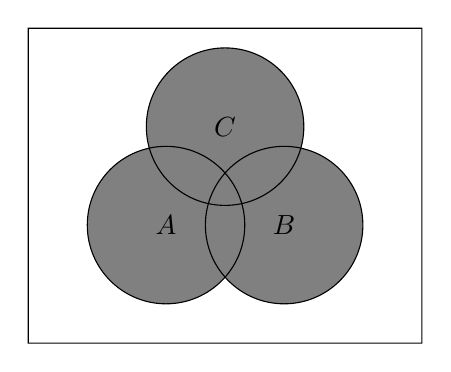
\begin{tikzpicture}[fill=gray]
\fill \B;
\fill \A;
\fill \C;
\draw \A (-0.75,0) node {$A$} 
	\B (0.75,0) node {$B$}
	\C (0,1.25) node{$C$}
      \R;
\end{tikzpicture}
\end{center}
\item at most one of the events $A,B,C,$ occurs $= [(A \cap B) \cup (A \cap C) \cup (B \cap C)]'$\\
\begin{center}
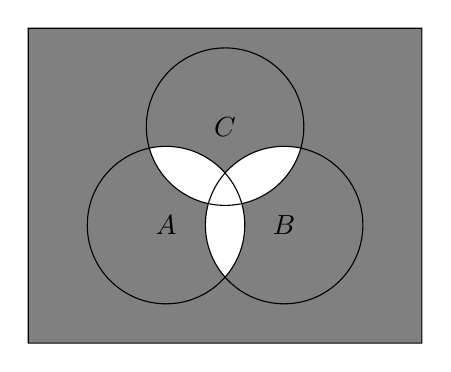
\begin{tikzpicture}
\fill[gray] \R;
\scope
	\clip \A;
	\fill[white] \B;
	\fill[white] \C;
\endscope
\scope
	\clip \C;
	\fill[white] \B;
\endscope
\draw \A (-0.75,0) node {$A$} 
	\B (0.75,0) node {$B$}
	\C (0,1.25) node{$C$}
      \R;
\end{tikzpicture}
\end{center}
\item none of the events $A,B,C$ occurs $= (A \cup B \cup C)'$
\begin{center}
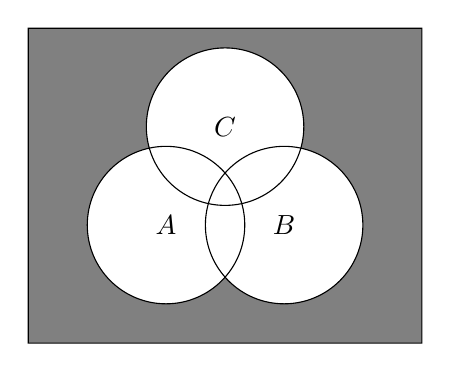
\begin{tikzpicture}[fill=gray]
\scope
	\clip \R % from rectangle
	\A; % clip A
	\scope
		\clip \R % from rectangle
		\B; % clip B
		\scope
			\clip \R % from rectangle
			\C; % clip C
			\fill \R;
		\endscope
	\endscope
\endscope
\draw \A (-0.75,0) node {$A$} 
	\B (0.75,0) node {$B$}
	\C (0,1.25) node{$C$}
      \R;
\end{tikzpicture}
\end{center}
\item all three events $A,B,C$ occur $= A \cap B \cap C$
\begin{center}
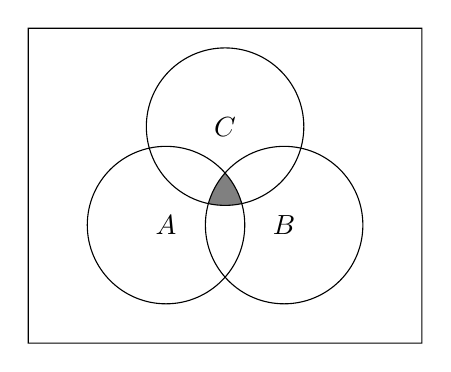
\begin{tikzpicture}[fill=gray]
\scope
\clip \A;
	\scope
		\clip \C;
		\fill \B;
	\endscope
\endscope
\draw \A (-0.75,0) node {$A$} 
	\B (0.75,0) node {$B$}
	\C (0,1.25) node{$C$}
      \R;
\end{tikzpicture}
\end{center}
\item exactly one of the events $A,B,C$ occur $= [A \cap (B \cup C)'] \cup [B \cap (A \cup C)'] \cup [C \cap (A \cup B)']$
\begin{center}
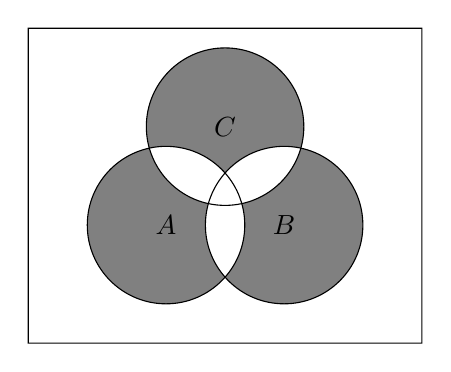
\begin{tikzpicture}
\fill[gray] \A;
\fill[gray] \B;
\fill[gray] \C;
\scope
	\clip \A;
	\fill[white] \B;
	\fill[white] \C;
\endscope
\scope
	\clip \B;
	\fill[white] \C;
\endscope
\draw \A (-0.75,0) node {$A$} 
	\B (0.75,0) node {$B$}
	\C (0,1.25) node{$C$}
      \R;
\end{tikzpicture}
\end{center}
\item events $A$ and $B$ occur but not $C = A \cap B \cap C'$
\begin{center}
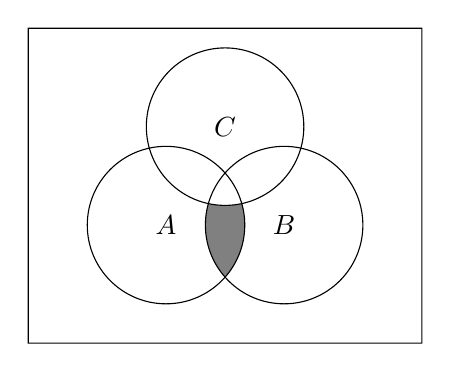
\begin{tikzpicture}
\scope
	\clip \A;
	\fill[gray] \B;
\endscope
\scope
	\clip \A;
	\clip \B;
	\fill[white] \C;
\endscope
\draw \A (-0.75,0) node {$A$} 
	\B (0.75,0) node {$B$}
	\C (0,1.25) node{$C$}
      \R;
\end{tikzpicture}
\end{center}
\item either event $A$ occurs or, if not, then $B$ also does not occur $= A \cup (A \cup B)'$
\begin{center}
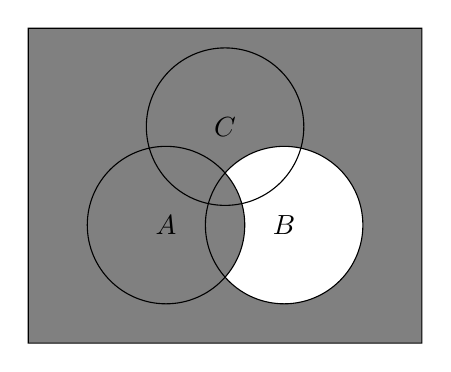
\begin{tikzpicture}
\fill[gray] \R;
\scope
	\clip \R
	\A;
	\fill[white] \B;
\endscope
\draw \A (-0.75,0) node {$A$} 
	\B (0.75,0) node {$B$}
	\C (0,1.25) node{$C$}
      \R;
\end{tikzpicture}
\end{center}
	\end{enumerate}
\pagebreak
\item You flip a fair coin 3 times. What is the probability of the following events assuming that all sequences are equally likely.
	\begin{enumerate}[label=\alph*)]
\item Three heads: HHH \[\bigg(\frac{1}{2}\bigg)^3 = \frac{1}{8}\]
\item Head, tail, head: HTH \[\bigg(\frac{1}{2}\bigg)^3 = \frac{1}{8}\]
\item Any sequence with two heads and 1 tail \[\frac{{{3}\choose{2}}}{2^3} = \frac{3}{8}\]
\item Any sequence with number of heads is greater than or equal to number of tails \[\frac{{{3}\choose{1}}}{2^3} + \frac{{{3}\choose{2}}}{2^3} = \frac{1}{8} + \frac{3}{8} = \frac{1}{2}\]
	\end{enumerate}
\item Alice and Bob each choose a random number in the interval [0,2]. We assume a uniform probability law under which the probability of an event is proportional to its area.\\
Find the probabilities $p(B),p(C),p(A\cap D)$ of the following events:
	\begin{enumerate}[label=$\Alph*$:]
\item The magnitude of the difference of two numbers is greater than $\frac{1}{3}$
\begin{center}
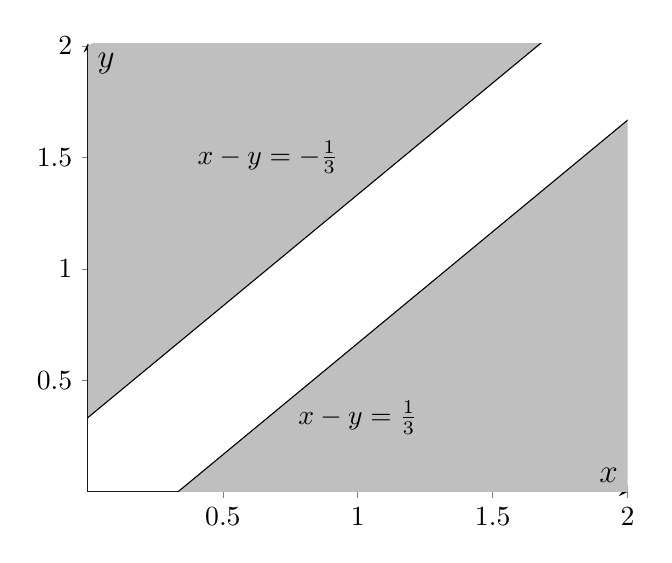
\begin{tikzpicture}
	\begin{axis}[
	axis lines=middle,
	xlabel={\large $x$},
	ylabel={\large $y$},
	xmin=0,
	xmax=2,
	ymin=0,
	ymax=2.01
	]
		\addplot [name path=A]{x+(1/3)};
		\addplot [name path=B]{x-(1/3)};
		\path[name path=xaxis] (axis cs:0,0) -- (axis cs:2,0);
		\path[name path=yaxis] (axis cs:0,0) -- (axis cs:0,2);
		\addplot [gray!50] fill between[of=xaxis and B];
		\addplot [gray!50] fill between[of=yaxis and A];
		\node at (axis cs:1,1/3) {$x-y=\frac{1}{3}$};
		\node at (axis cs:2/3,3/2) {$x-y=-\frac{1}{3}$};
	\end{axis}
\end{tikzpicture}
\end{center}
The area of the square made of points $(0,0),(2,0),(0,2),(2,2)$ represents the total sample space.
\[p(A)=\frac{(2-\frac{1}{3})^2}{4} = \bigg(\frac{25}{9}\bigg)\bigg(\frac{1}{4}\bigg)=\frac{25}{36}\]
\item At least one of the numbers is greater than $\frac{1}{3}$
\begin{center}
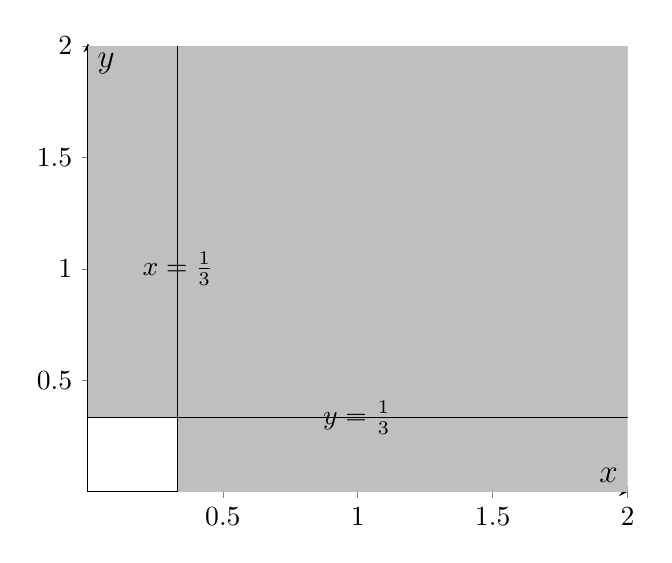
\begin{tikzpicture}
	\begin{axis}[
	axis lines=middle,
	xlabel={\large $x$},
	ylabel={\large $y$},
	xmin=0,
	xmax=2,
	ymin=0,
	ymax=2.01
	]
		\addplot [name path=C] coordinates {(1/3,0)(1/3,2)};
		\addplot [name path=D] coordinates {(0,1/3)(2,1/3)};
		\path[name path=xlimit] (axis cs:2,0) -- (axis cs:2,2);
		\path[name path=ylimit] (axis cs:0,2) -- (axis cs:2,2);
		\addplot [gray!50] fill between[of=C and xlimit];
		\addplot [gray!50] fill between[of=D and ylimit];
		\node at (axis cs:1,1/3) {$y=\frac{1}{3}$};
		\node at (axis cs:1/3,1) {$x=\frac{1}{3}$};
	\end{axis}
\end{tikzpicture}
\end{center}
\[p(B)=2^2-\bigg(\frac{1}{3}\bigg)^2=4-\frac{1}{9}=\frac{35}{9}\]
\item The two numbers are equal
\begin{center}
\begin{tikzpicture}
	\begin{axis}[
	axis lines=middle,
	xlabel={\large $x$},
	ylabel={\large $y$},
	xmin=0,
	xmax=2,
	ymin=0,
	ymax=2.01
	]
		\addplot [name path=C]{x};
		\node at (axis cs:1,1) {$y=x$};
	\end{axis}
\end{tikzpicture}
\end{center}
\[p(C)=0 \ \text{since there is no area}\]
\item Alice's number is greater than $\frac{1}{3}$
\begin{center}
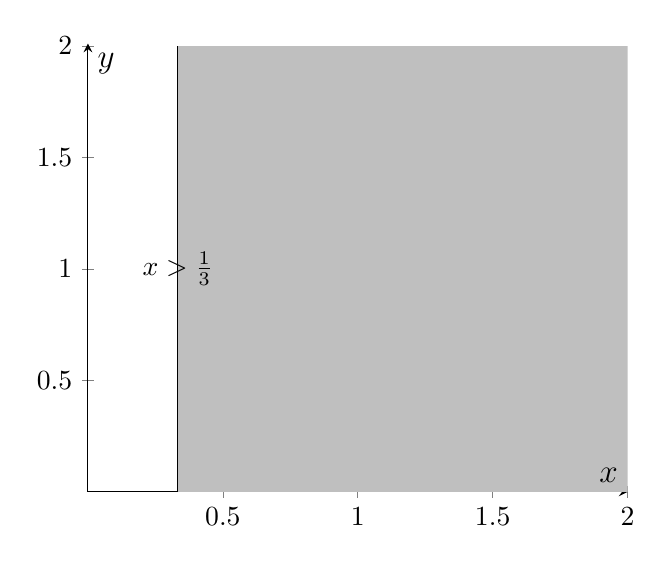
\begin{tikzpicture}
	\begin{axis}[
	axis lines=middle,
	xlabel={\large $x$},
	ylabel={\large $y$},
	xmin=0,
	xmax=2,
	ymin=0,
	ymax=2.01
	]
		\addplot [name path=C] coordinates {(1/3,0)(1/3,2)};
		\path[name path=xlimit] (axis cs:2,0) -- (axis cs:2,2);
		\addplot [gray!50] fill between[of=C and xlimit];
		\node at (axis cs:1/3,1) {$x>\frac{1}{3}$};
	\end{axis}
\end{tikzpicture}
\end{center}
\[p(D) = 2^2 - \bigg(2-\frac{1}{3}\bigg)^2 = 4-\bigg(\frac{5}{3}\bigg)^2=\frac{11}{9}\]
\begin{center}
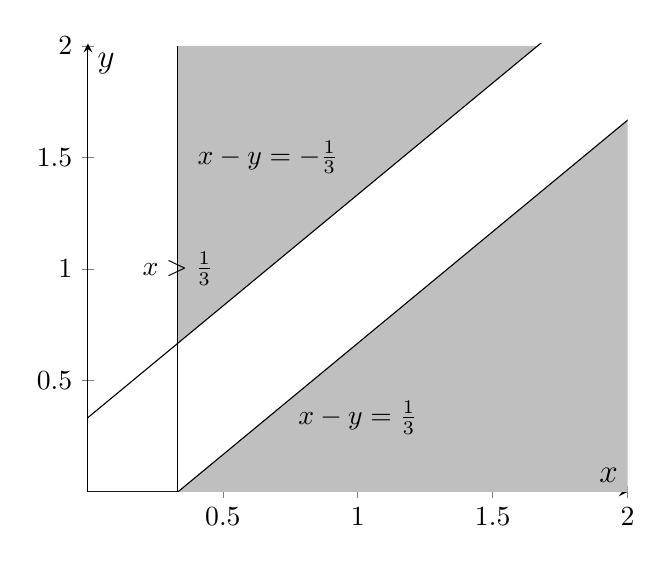
\begin{tikzpicture}
	\begin{axis}[
	axis lines=middle,
	xlabel={\large $x$},
	ylabel={\large $y$},
	xmin=0,
	xmax=2,
	ymin=0,
	ymax=2.01
	]
		\addplot [name path=A]{x+(1/3)};
		\addplot [name path=B]{x-(1/3)};
		\path[name path=xaxis] (axis cs:0,0) -- (axis cs:2,0);
		\path[name path=yaxis] (axis cs:0,0) -- (axis cs:0,2);
		\path[name path=topline] (axis cs:1/3,2/3) -- (axis cs:5/3,2);
		\addplot [gray!50] fill between[of=xaxis and B];
		\node at (axis cs:1,1/3) {$x-y=\frac{1}{3}$};
		\node at (axis cs:2/3,3/2) {$x-y=-\frac{1}{3}$};
		\addplot [name path=C] coordinates {(1/3,0)(1/3,2)};
		\path[name path=xlimit] (axis cs:2,0) -- (axis cs:2,2);
		\addplot [gray!50] fill between[of=C and topline];
		\node at (axis cs:1/3,1) {$x>\frac{1}{3}$};
	\end{axis}
\end{tikzpicture}
\end{center}
\[p(A \cap D) = 2^2 - \frac{\frac{5}{3}^2}{2} - \bigg(\frac{4}{3}\bigg)\bigg(\frac{5}{3}\bigg)\bigg(\frac{1}{2}\bigg) = 4-\frac{25}{18}-\frac{20}{18}=\frac{3}{2}\]
	\end{enumerate}
\item Mike and John are playing a friendly game of darts where the dart board is a disk with radius of 10 in.\\
Whenever a dart falls within 1 in. of the center, 50 points are scored. If the point of impact is between 1 and 3 in. from the center, 30 points are scored, if it is a distance of 3 to 5 in., 20 points are scored and if it is further than 5 in., 10 points are scored.\\
Assume that both players are skilled enough to be able to throw the dart within the boundaries of the board. Mike can place the dart uniformly on the board (i.e., the probability of the dart falling in a given region is proportional to its area).
	\begin{enumerate}[label=\alph*)]
\item What is the probability that Mike scores 50 points on one throw?
\[\frac{\pi^2}{100\pi^2}=\frac{1}{100}\]
\item What is the probability of him scoring 30 points on one throw?
\[\frac{3^2\pi-\pi^2}{100\pi^2}=\frac{8\pi^2}{100\pi^2}=\frac{2}{25}\]
	\end{enumerate}
\end{enumerate}
\pagebreak

%%%%% CONDITIONAL PROBABILITY AND BAYES' RULE %%%%%

\section{Conditional Probability and Bayes' Rule}
\begin{enumerate}[label=\textbf{Problem \arabic*.}]
\item Assume that each memory bank which is equally likely to be used for storing data or for storing instructions. If a computer system has two memory banks, what is the probability that both are for storing data given (a) the first one is used for storing data, (b) at least one is for storing data?\\
$P[n^{th}$ bank stores data$]=p(D_n)=\frac{1}{2}$
	\begin{enumerate}[label=\alph*)]
\item \[P[D_1D_2|D_1] = \frac{P[D_1D_2 \cap D_1]}{P[D_1]} = \frac{P[D_1D_2]}{P[D_1]}=\frac{\frac{1}{2}\frac{1}{2}}{\frac{1}{2}}=\frac{\frac{1}{4}}{\frac{1}{2}}=\frac{1}{2}\]
\item \[P[D_1D_2|D] = \frac{P[D|D_1D_2]P[D]}{P[D_1D_2]} = \frac{\frac{1}{4}}{\frac{3}{4}}=\frac{1}{3}\]
	\end{enumerate}
\item In the design of digital circuit, the multiplexer (MUX) are used to select an input from a set of inputs, now suppose that you have a three-input MUX, the first input is always connected to high level voltage (binary signal one), the second input has a value either 1 or 0 with equal probability ($\frac{1}{2}$ for each case), and third input is connected to another logical gate which outputs a value 1 with probability $\frac{3}{4}$. When the output of MUX shows a value of 1, then what is the probability that the first input is passed to the output of the MUX?
\[P[I_1|1]=\frac{P[1|I_1]P[I_1]}{P[1]}=\frac{1\big(\frac{1}{3}\big)}{\frac{1+\frac{1}{2}+\frac{3}{4}}{3}}=\frac{\frac{1}{3}}{\frac{3}{4}}=\frac{4}{9}\]
\item CPU (Central Processing Unit) and GPU (Graphics Processing Unit) are using a single data bus together to transfer data to each other. Both may request the bus at the same time. Suppose CPU may be granted with probability 0.7, whereas GPU, independently, may be granted with probability 0.4.
	\begin{enumerate}[label=\alph*)]
\item Given that exactly one request to data bus is granted, what is the probability that it was GPU's request?
\[P(GPU|G)=\frac{P(G|GPU)P(GPU)}{P(G)}=\frac{0.4\big(\frac{1}{2}\big)}{\frac{0.7+0.4}{2}}=\frac{4}{11}\]
\item Given that the request is granted, what is the probability that GPU is granted? (ignore that there could be a conflict if both CPU and GPU are granted)
\[P(GPU|G)=\frac{P(G|GPU)P(GPU)}{P(G)}=\frac{1(0.4)}{\frac{0.7+0.4}{2}}=\frac{8}{11}\]
	\end{enumerate}
\item Oscar has lost his dog in either forest $A$ (with a priori probability 0.4) or in forest $B$ (with a priori probability 0.6).\\
On any given day, if the dog is in $A$ and Oscar spend a day searching for it in $A$, the conditional probability that he will find the dog that day is 0.25. Similarly, if the dog is in $B$ and Oscar spends a day looking for it there, the conditional probability that he will find the dog that day is 0.15.\\
The dog cannot go from one forest to another. Oscar can search only in the daytime and he can travel from one forest to the other only at night.
	\begin{enumerate}[label=\alph*)]
	\item In which forest should Oscar look to maximize the probability he finds his dog on the first day of the search?\\
	Forest $A$, since the conditional probability that he will find it in that forest is higher than $B$.
	\item Given that Oscar looked in $A$ on the first day but didn't find his dog, what is the probability that the dog is in $A$?\\
	\[P(D_A|F_A')=\frac{P[F_A'|D_A]P[D_A]}{P[F_A']}=\frac{\big(\frac{3}{4}\big)\big(\frac{4}{10}\big)}{1-\big(\frac{4}{10}\big)\big(\frac{1}{4}\big)}=\frac{\frac{3}{10}}{\frac{9}{10}}=\frac{1}{3}\]
	\item If Oscar flips a fair coin to determine where to look on the first day and finds the dog on the first day, what is the probability that he looked in $A$?
	\[\frac{1}{2}\]
	\end{enumerate}
\item In this problem, you will develop an algorithm for classifying whether an email message is spam/non-spam. Assuming that from all emails only 20\% are spam and for simplicity, occurence of each word in an email is independent from other words in the same message. What is the probability of the following messages to be spam?
\begin{center}
\begin{tabular}{ |c|c|c| }
\hline 
\textbf{word} & $p(word|spam)$ & $p(word|nonspam)$ \\
\hline
Hello & 0.8 & 0.9 \\
\hline
Money & 0.95 & 0.02 \\
\hline
send & 0.9 & 0.2 \\
\hline
friend & 0.02 & 0.3 \\
\hline
party & 0.17 & 0.42 \\
\hline
Let's & 0.4 & 0.6 \\
\hline
\end{tabular}
\end{center}
	\begin{enumerate}[label=\alph*)]
	\item ``Hello Friend Send Money''
	\[P[S|H]=\frac{P[H|S]}{P[H|S]+P[H|S']}=\frac{0.8}{0.8+0.9}=\frac{8}{17}\]
	\[P[S|F]=\frac{P[F|S]}{P[F|S]+P[F|S']}=\frac{0.02}{0.02+0.3}=\frac{1}{16}\]
	\[P[S|s]=\frac{P[s|S]}{P[s|S]+P[s|S']}=\frac{0.9}{0.9+0.2}=\frac{9}{11}\]
	\[P[S|M]=\frac{P[M|S]}{P[M|S]+P[M|S']}=\frac{0.95}{0.95+0.02}=\frac{95}{97}\]
	\[P[S]=\frac{P[S|H]P[S|F]P[S|s]P[S|M]}{P[S|H]P[S|F]P[S|s]P[S|M]+(1-P[S|H])(1-P[S|F])(1-P[S|s])(1-P[S|M])}=\frac{38}{41}\]
	\item ``Hello Friend Let's Party''
	\[P[S|H]=\frac{P[H|S]}{P[H|S]+P[H|S']}=\frac{0.8}{0.8+0.9}=\frac{8}{17}\]
	\[P[S|F]=\frac{P[F|S]}{P[F|S]+P[F|S']}=\frac{0.02}{0.02+0.3}=\frac{1}{16}\]
	\[P[S|L]=\frac{P[L|S]}{P[L|S]+P[L|S']}=\frac{0.4}{0.4+0.6}=\frac{4}{10}\]
	\[P[S|P]=\frac{P[P|S]}{P[P|S]+P[P|S']}=\frac{0.17}{0.17+0.42}=\frac{17}{59}\]
	\[P[S]=\frac{P[S|H]P[S|F]P[S|L]P[S|P]}{P[S|H]P[S|F]P[S|L]P[S|P]+(1-P[S|H])(1-P[S|F])(1-P[S|L])(1-P[S|P])}=\frac{136}{8641}\]
	\end{enumerate}
\end{enumerate}
\pagebreak

%%%%% PROBABILITY DISTRIBUTIONS %%%%%

\section{Probability Distributions}
\begin{enumerate}[label=\textbf{Problem \arabic*.}] 
\item Alice plays with Bob the following game: first Alice randomly chooses 4 cards out of a 52-card deck, memorizes them, and places them back into the deck. Then Bob randomly chooses 8 cards out of the same deck. Alice wins if Bob's cards include all cards selected by her. What is the probability of this happening?
\[\frac{{{4}\choose{4}}{{48}\choose{4}}}{{{52}\choose{8}}}\]
\item We need to download a short video clip over the Internet. The video clip contains 200 frames and each frame is cut into 8 packets to send. Each packet has a probability of $p$ to be lost. Assume that each frame can be successfully decoded only when there are at least 6 packets received; and the video can play only when 90\% of frames can be decoded. What is the probability that the video downloaded can be played?\\
$P[$successfully decode frame$]=P[F]\\
P[$video is playable$]=P[P]\\$
\[P[F]={{8}\choose{6}}p^2(1-p)^6+{{8}\choose{7}}p(1-p)^7+{{8}\choose{8}}(1-p)^8\]
\[P[P]=\sum_{i=180}^{200}{{200}\choose{i}}P[F]^i(1-P[F])^{200-i}\]
\item The number of tasks coming per minute into a CPU is Poisson random variable with parameter 3.
	\begin{enumerate}[label=\alph*)]
	\item Find the probability that no tasks come in a given 1 minute period
	\[e^{-3}\frac{3^0}{0!}=e^{-3}\]
	\item Assume that the number of tasks arriving in two different minutes are independent. Find the probability that at least 2 tasks will arrive in a given 2 minute period
	\[1-e^{-6}-6e^{-6}\]
	\end{enumerate}
\end{enumerate}

\end{document}